\documentclass{article}
\usepackage{indentfirst}     
\usepackage{setspace}        
\usepackage[top=1in, bottom=1in, left=1.25in, right=1.25in]{geometry} 
\usepackage{amsmath}
\usepackage{color}
\usepackage{graphicx}
\usepackage{float}
\usepackage{fancyhdr}
\usepackage{hyperref}
\usepackage{mathtools}
\usepackage{amsfonts}
\usepackage{subcaption}


\title{Note on Transition Dynamics\\ (MIT Shocks)}
\author{Yanran Guo}
\date{Oct. 2019} 
\begin{document}
\begin{spacing}{1.5}
\maketitle

\section*{Overview}
The purpose of this note is to explain the details of the computation of the deterministic transition dynamics of the Aiyagari (1994) model after an unexpected permanent shock. Such unforeseen aggregate shocks are called ``MIT shocks''. As an example, I assume the shock is a change in borrowing constraint. In particular, borrowing constraint increases from $\phi$ to $\phi'$.

\begin{itemize}
\item When MIT shocks hit the economy, we can compute the stationary equilibria before and after the shock. Then we can make comparison between the two steady state. However this approach can only assess the starting point and the end point. What happens in between remains unclear. Hence we need to compute the whole transition: the shock will change the household consumption/saving and possibly labor supply decision (if there is endogenous labor supply), hence aggregate prices, and will induce dynamics away from the current stationary equilibrium towards the new one.
\item The transition is characterized by a sequence of aggregate prices and quantities. Notice that prices $(r, w)$ are time-varying during transition.
\item The transition dynamics induced by MIT shocks are \textcolor{red}{deterministic}. Since we know the exact new value for e.g. borrowing constraint, we know there will be a deterministic path for prices and for the distribution of household type $\mu$. Therefore, we do not need to keep track of the distribution as an additional state, as time is a sufficient statistic. When there is aggregate uncertainty (e.g. Krusell and Smith, 1998), the distribution $\mu$ becomes an aggregate state.
\end{itemize}
\newpage



%%%%%%%%%%%%%%%%%%%%%%%%%%%%%%%%%%%%%%%%%%%%%%%%%%%%%%%%%%%%%%%%%%%%%%%%%%%
\section{Computation Algorithm}
\setlength{\parindent}{2em}
\begin{enumerate}
\item Compute the initial steady state ($\phi$) and the final steady state ($\phi'$). Set the initial steady state as $t=0$ steady state. And the final steady state as $t=T$ steady state. Hence there are $T-1$ periods during the transition.
\item Choose a time $T$ at which point we assume the economy has reached the new steady state. $t=1$ is the period when the unexpected change in $\phi$ happened, and $t=T$ is sufficiently far in future so that we can safely assume that by time $T$ the economy is in the new steady state.
\item Guess a path for aggregate capital $\Big(\{K_t\}_{t=1}^{T-1}\Big)^0$. 
\item Given $\Big(\{K_t\}_{t=1}^{T-1}\Big)^0$, solve for sequences of prices, $\{r_t\}_{t=1}^{T-1}$ and $\{w_t\}_{t=1}^{T-1}$, using firm FOCs. \\
Notice that the aggregate labor supply can be computed exogenously in the stationary equilibrium. If we store the stationary distribution regarding the idiosyncratic shocks as $\{P_i\}_{i=1}^{n}$, the aggregate labor supply in the stationary distribution can be computed as
\begin{align*}
N=\sum_{i=1}^ns_iP_i
\end{align*}
Hence $r$ and $w$ are functions of $K$.
\item Backward Induction:\\
Assume that at $t=T$, the economy is in the new steady state. Since we already computed the new steady state in Step-1, we know the value function in the last period $t=T$. That means we know $V(k_T,s_T)$ in $t=T-1$ Bellman equation
\begin{align*}
V(k_{T-1},s_{T-1})=max_{c_{T-1},k_{T}}\Big\{ \ u(c)+\beta\sum_{s'}\pi(s'|s)V(k_T,s_T)\Big\}
\end{align*}
Hence we can solve the value function in period $t=T-1$. Similarly, given $V(k_{T-1},s_{T-1})$, we can solve value function in period $T-2$.\\
In summary, in this step, we solve the value function backwards from $t=T-1,...,1$, setting $V_T=V_{ss_{new}}$. Hence we obtain a sequence of value functions $\{V_t\}_{t=1}^{T-1}$ 
\item Forward Calculation:\\
$t=1$ is the period when the unexpected change in $\phi$ happened. Hence in $t=0$, the economy is still in its initial steady state. Since we already computed the initial steady state in Step-1, we know the policy function $k'$ and distribution $\mu$ in period $t=0$. 
\begin{enumerate}
\item Using law of motion for $\mu$, compute $\mu$ in period $t=1$
\begin{align*}
\mu(k_1,s_1)=\sum_{k_0}\sum_{s_0}\mu(k_0,s_0)\pi(s_1|s_0)\textbf{1}_{k_1=g(k_0,s_0)}
\end{align*}
\item Given the sequence of $r_t$ and $w_t$, we know $r$ and $w$ in period $t=1$. Given the sequence of value functions, we know value function in period $t=2$. Using Bellman equation, solve the policy function in period $t=1$, which is $k_1$.
\item With distribution $\mu_1$ and policy function $k_1$, compute the aggregate capital supply $K^s_1$
\item Define the excess capital demand $K_1-K^s_1$.
\item $K^s_1$ is computed using policy function $g_k(k,s)$ and stationary distribution $\mu_0$, which are computed given prices. And since the prices are functions of aggregate capital $K_1$, hence $K^s_1$ depends on $K_1$. Therefore, $\Phi=K_1-K^s_1$ is a function of $K_1$. Then use `fsolve' to get the the solution for $K^*_1$
\item Keep doing this for each following period until $t=T-1$. We get a sequence of $\{K^*_t\}_{t=1}^{T-1}$
\end{enumerate}
\item Compute the maximum difference between $\{K^*_t\}_{t=1}^{T-1}$ and our guess $\Big(\{K_t\}_{t=1}^{T-1}\Big)^0$
\item If the difference is below tolerance level, stop.
\item Otherwise, update guess
\begin{align*}
\Big(\{K_t\}_{t=1}^{T-1}\Big)^1=\nu\Big(\{K_t\}_{t=1}^{T-1}\Big)^0+(1-\nu)\{K_t^*\}_{t=1}^{T-1}, \ \ \ \ \ \ \nu\in(0,1)
\end{align*}
and go to Step-2
\end{enumerate}

\newpage
\subsection*{A summary of the functions I used to compute the transition dynamics}
\begin{figure}[!htb]
\centering
\hspace*{2cm}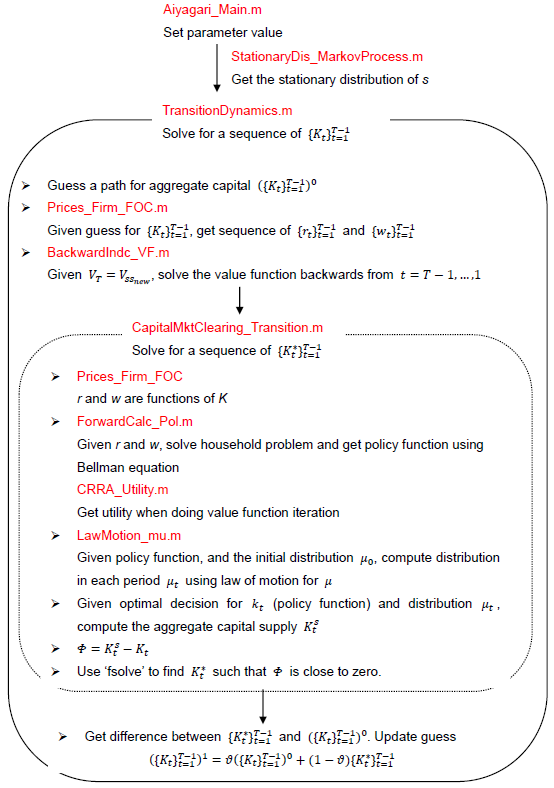
\includegraphics[width=\textwidth,natwidth=400,natheight=400]{readme2.png}\hspace*{-2cm}\\
\end{figure}


\newpage
\section*{Appendix: Another Way to Compute Transition Dynamics}
\setlength{\parindent}{2em}
\begin{enumerate}
\item Choose a time $T$ at which point we assume the economy has reached new steady state.
\item Guess a path for aggregate capital demand $\Big(\{K_t\}_{t=1}^{T-1}\Big)^0$. 
\item Given $\Big(\{K_t\}_{t=1}^{T-1}\Big)^0$, solve for sequences of prices, $\{r_t\}_{t=1}^{T-1}$ and $\{w_t\}_{t=1}^{T-1}$, using firm FOCs.
\item Solve the value function and policy function backwards from $t=T-1,...,1$, setting $V_T=V_{ss_{new}}$.
\item Starting from the initial steady state distribution, simulate the distribution forward from $t=1,...T-1$ using the policy function and idiosyncratic productivity Markov transition matrix.
\item At each $t$, compute aggregate capital supplied $K^s_t$ using distribution and policy functions.
\item Compute the maximum difference between supply and demand $\xi=max|K_t-K^s_t|$
\item If $\xi<$tolerance level, stop.
\item Otherwise, update guess
\begin{align*}
\Big(\{K_t\}_{t=1}^{T-1}\Big)^1=\nu\Big(\{K_t\}_{t=1}^{T-1}\Big)^0+(1-\nu)\{K_t^s\}_{t=1}^{T-1}, \ \ \ \ \ \ \nu\in(0,1)
\end{align*}
and go to Step-2
\end{enumerate}














\end{spacing}
\end{document}